
\documentclass[10pt,a4paper]{article}
\usepackage[margin=1.45cm]{geometry}
\usepackage[T1]{fontenc}
\usepackage{microtype}
\usepackage{fancyhdr}
\usepackage{graphicx}
\usepackage{booktabs}
\usepackage{amsmath}
\usepackage{amssymb}
\usepackage{caption}
\usepackage{subcaption}
\usepackage{float}
\usepackage{hyperref}
\usepackage{enumitem}
\setlist{nosep,leftmargin=*}
\setlength{\parindent}{0pt}
\setlength{\parskip}{3pt}
\captionsetup{font=small}
\title{\textbf{Optimization Methods for Polynomial Regression}\\\large Retail Demand Forecasting Case Study}
\author{\begin{tabular}{c}\textbf{Mohamed Elhadidy}\\ Matriculation Number: 12328710\\ Optimization for Data Science - Final Project\end{tabular}}
\date{SS 2026}

\pagestyle{fancy}
\fancyhf{}
\lhead{Polynomial Regression for Demand Forecasting}
\rhead{Mohamed Elhadidy}
\cfoot{\thepage}
\setlength{\headheight}{12pt}

\begin{document}
\maketitle
\thispagestyle{plain}

\begin{center}
\fbox{\begin{minipage}{0.92\textwidth}
\textbf{Summary.} This report implements polynomial regression for a demand forecasting case study and compares deterministic, stochastic, accelerated, proximal, and adaptive optimization methods under smooth, strongly convex, non-smooth, and non-convex objective structures.
\end{minipage}}
\end{center}

\section{Application and data}
The application is daily retail demand forecasting. I used the Kaggle Store Item Demand Forecasting data and focused on one clean time series: store 1, item 1. The full training file has 913000 rows; after selecting the store-item pair and dropping rows needed for lag features, the experiment used 1454 training observations from 2013--2016 and 365 test observations from 2017. The target is daily sales.

The raw engineered features were: \texttt{t}, \texttt{day\_of\_week}, \texttt{month}, \texttt{day\_of\_year}, \texttt{weekend}, \texttt{lag\_1}, \texttt{lag\_7}, \texttt{rolling\_mean\_7}. These features were standardized using training-set statistics only. The target was also standardized during optimization, and RMSE/MAE were converted back to sales units for reporting. Polynomial features were generated from all monomials up to degree $p$; the main comparison used $p=3$, giving 165 parameters including the intercept.

\section{Polynomial regression objectives}
For design matrix $X\in\mathbb{R}^{n\times d}$ and target $y\in\mathbb{R}^n$, the prediction is $\hat y=Xw$. I compared four objective structures:
\begin{align*}
J_{\mathrm{mse}}(w) &= \frac{1}{2n}\|Xw-y\|_2^2 && \text{smooth convex},\\
J_{\mathrm{ridge}}(w) &= \frac{1}{2n}\|Xw-y\|_2^2 + \frac{\lambda}{2}\|w_{1:}\|_2^2 && \text{smooth strongly convex for }\lambda>0,\\
J_{\mathrm{lasso}}(w) &= \frac{1}{2n}\|Xw-y\|_2^2 + \lambda\|w_{1:}\|_1 && \text{convex non-smooth},\\
J_{\mathrm{nc}}(w) &= \frac{1}{2n}\|Xw-y\|_2^2 + \lambda\sum_{j>0}\left(1-e^{-w_j^2/(2\tau^2)}\right) && \text{smooth non-convex}.
\end{align*}
The intercept $w_0$ was not regularized. The smooth objectives used gradients implemented directly in NumPy. The L1 objective used the proximal operator, i.e. soft-thresholding, so ISTA/FISTA can handle the non-smooth term.

\section{Optimization algorithms}
The implemented algorithms were: Gradient Descent, Nesterov acceleration, Heavy Ball, SGD, SAGA, Adagrad, Adam, ISTA and FISTA. Gradient Descent and Nesterov used a step based on the Lipschitz estimate $L=\|X\|_2^2/n+\lambda$. SGD/Adagrad/Adam used mini-batches of 32 samples. SAGA used a stored table of individual gradients. Adam and Adagrad were included as adaptive stochastic methods beyond the basic deterministic methods.

\begin{figure}[H]
\centering
\begin{subfigure}{0.49\textwidth}
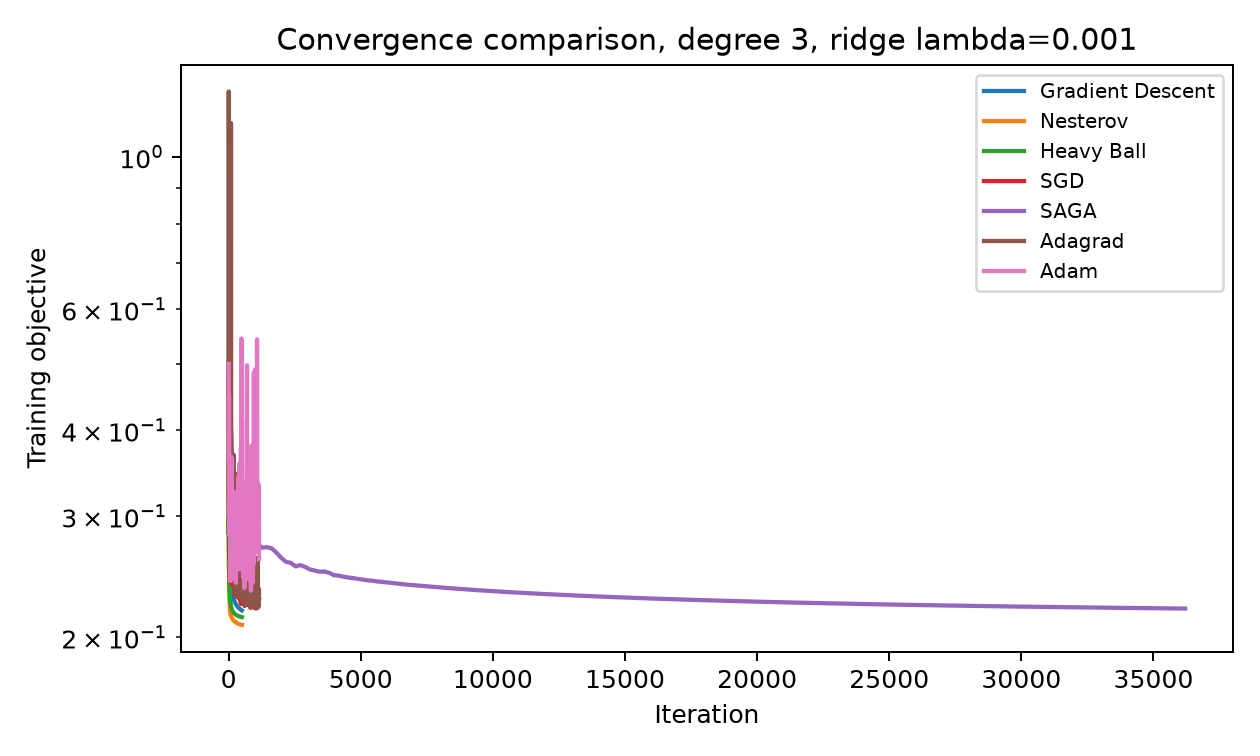
\includegraphics[width=\linewidth]{../figures/fig1_algorithm_convergence.png}
\caption{Training objective convergence.}
\end{subfigure}
\begin{subfigure}{0.49\textwidth}
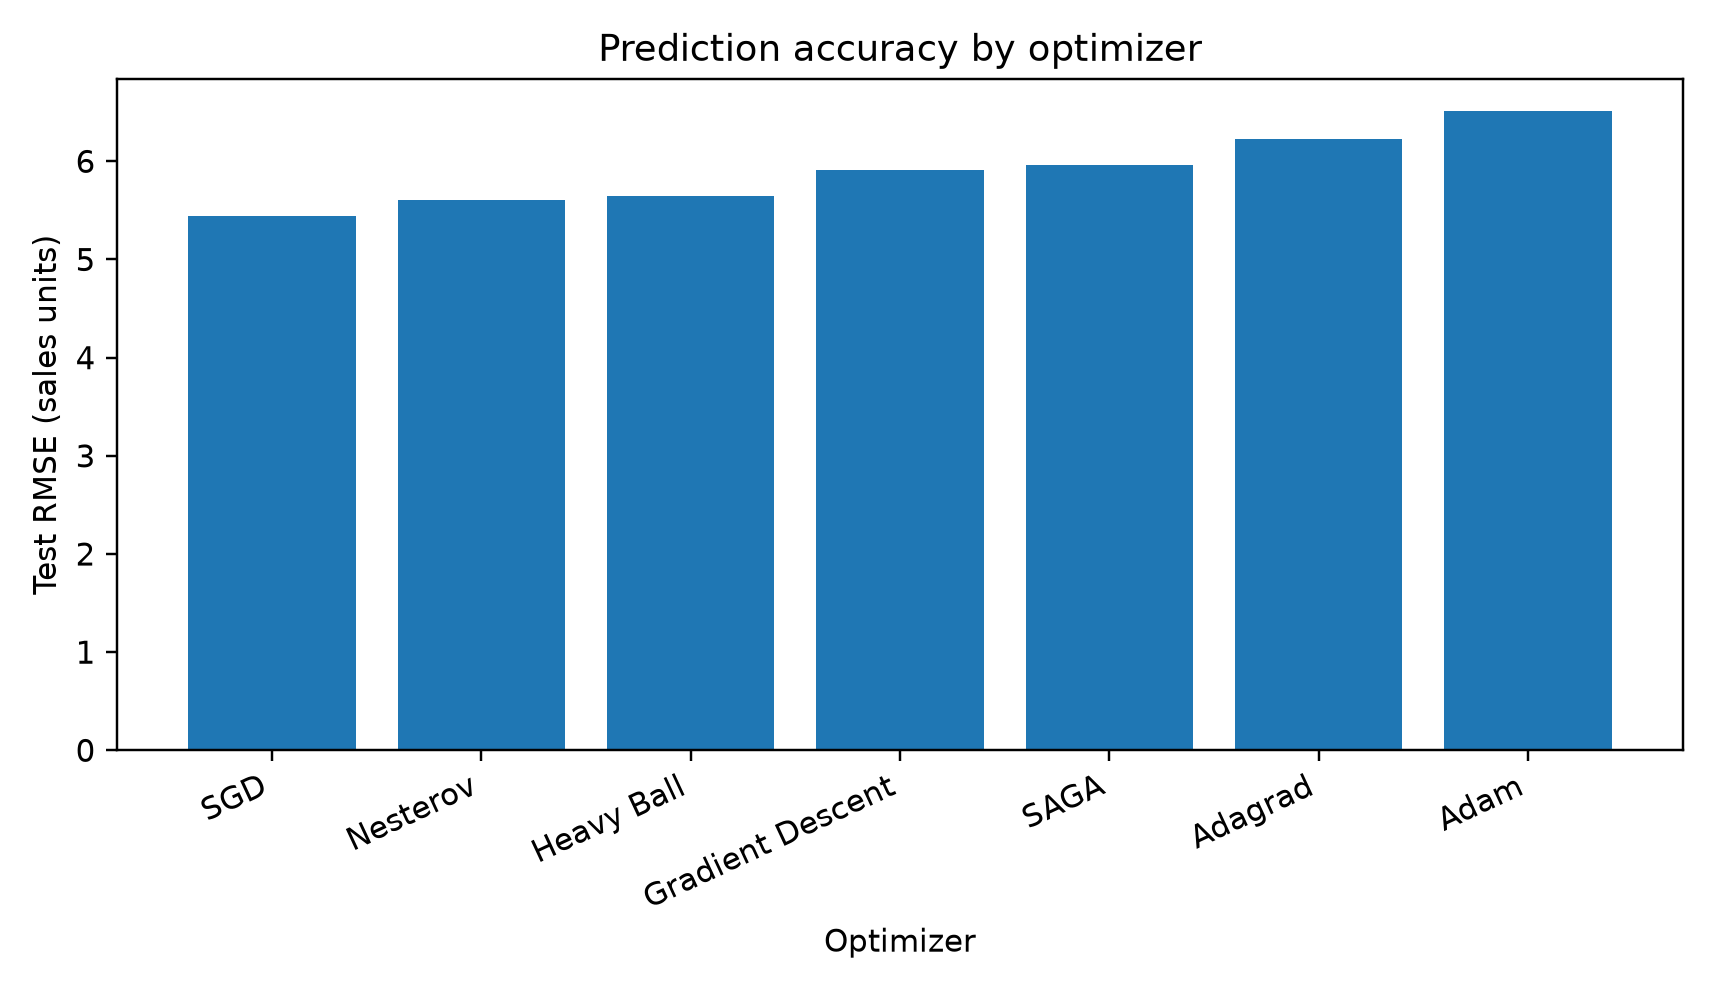
\includegraphics[width=\linewidth]{../figures/fig2_test_rmse_by_algorithm.png}
\caption{Test RMSE by optimizer.}
\end{subfigure}
\caption{Optimizer comparison for ridge polynomial regression with degree 3 and $\lambda=10^{-3}$.}
\end{figure}

\begin{table}[H]
\centering
\scriptsize
\caption{Main optimizer comparison. Lower test RMSE is better.}
\begin{tabular}{lrrr}
\toprule
Method & Train RMSE & Test RMSE & Test MAE\\
\midrule
SGD & 4.47 & 5.45 & 4.31 \\
Nesterov & 4.23 & 5.61 & 4.42 \\
Heavy Ball & 4.29 & 5.64 & 4.47 \\
Gradient Descent & 4.34 & 5.91 & 4.70 \\
SAGA & 4.36 & 5.97 & 4.74 \\
Adagrad & 4.43 & 6.22 & 4.97 \\
Adam & 4.73 & 6.51 & 5.00 \\
\bottomrule
\end{tabular}
\end{table}

\section{Experimental results}
The best test RMSE in the main optimizer comparison was obtained by SGD with RMSE $5.45$ and MAE $4.31$ sales units. Deterministic accelerated methods reached lower training objective faster than plain Gradient Descent, while the stochastic method gave the best validation accuracy in this finite-run experiment.

\begin{table}[H]
\centering
\scriptsize
\caption{Objective-structure comparison.}
\begin{tabular}{llrr}
\toprule
Objective & Method & Test RMSE & Final scaled MSE\\
\midrule
MSE & GD & 5.91 & 0.219 \\
MSE + L2 & Nesterov & 5.61 & 0.208 \\
MSE + L1 & FISTA & 5.46 & 0.212 \\
MSE + smooth L0-like & GD & 5.84 & 0.219 \\
\bottomrule
\end{tabular}
\end{table}

For polynomial degree, performance improved from degree 1 to degree 2 and then overfitted for higher degrees. This is expected because the number of parameters grows quickly relative to the single store-item time series. The best degree by test RMSE was degree 2. For L2 regularization, the best tested value was $\lambda=0.01$.

\begin{figure}[H]
\centering
\begin{subfigure}{0.49\textwidth}
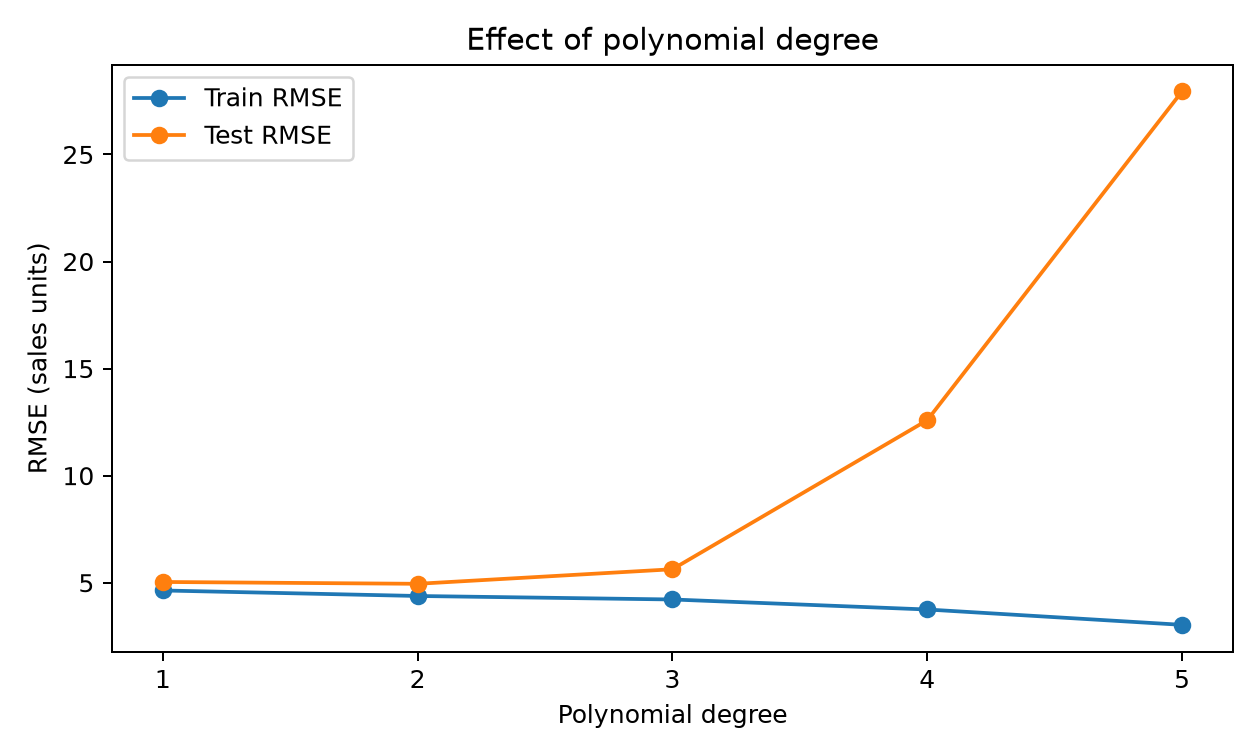
\includegraphics[width=\linewidth]{../figures/fig5_degree_effect.png}
\caption{Polynomial degree effect.}
\end{subfigure}
\begin{subfigure}{0.49\textwidth}
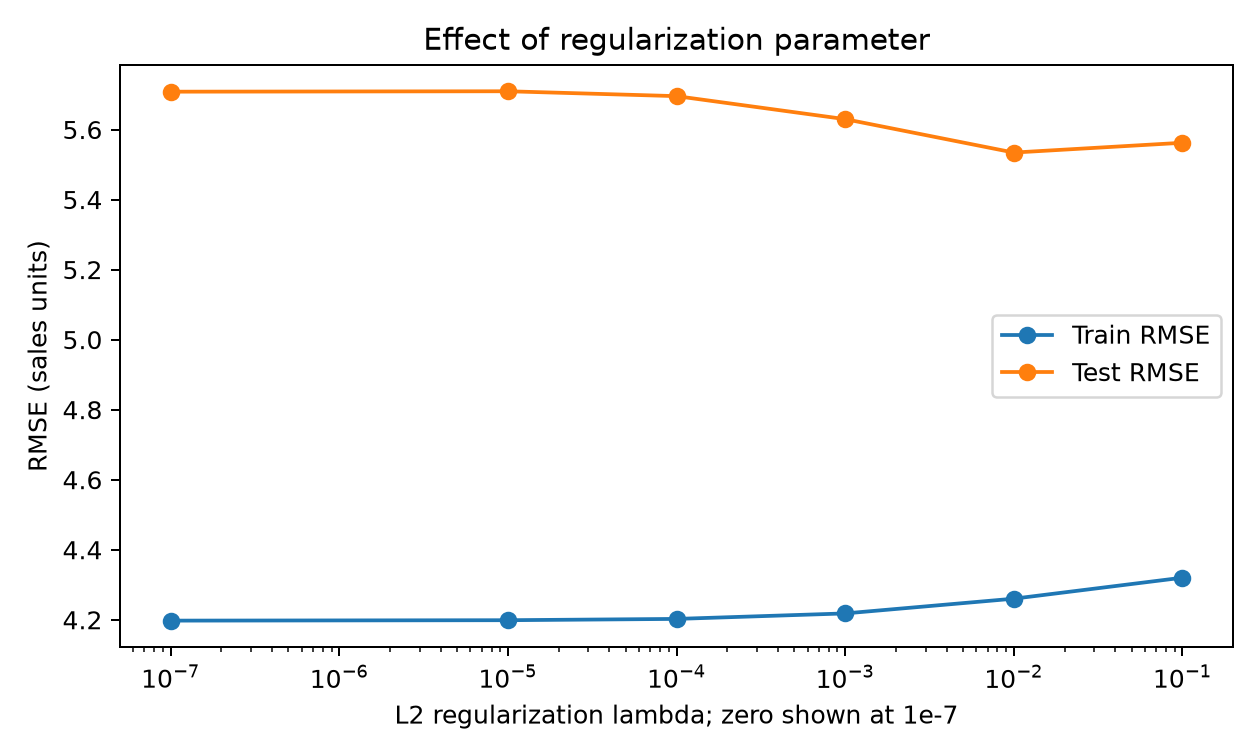
\includegraphics[width=\linewidth]{../figures/fig7_regularization_effect.png}
\caption{Regularization effect.}
\end{subfigure}
\caption{Hyperparameter effects required by the task.}
\end{figure}

\begin{table}[H]
\centering
\scriptsize
\caption{Polynomial degree effect using ridge reference solutions.}
\begin{tabular}{rrrr}
\toprule
Degree & Parameters & Train RMSE & Test RMSE\\
\midrule
1 & 9 & 4.64 & 5.04 \\
2 & 45 & 4.38 & 4.95 \\
3 & 165 & 4.22 & 5.63 \\
4 & 495 & 3.75 & 12.59 \\
5 & 1287 & 3.03 & 27.94 \\
\bottomrule
\end{tabular}
\end{table}

\begin{figure}[H]
\centering
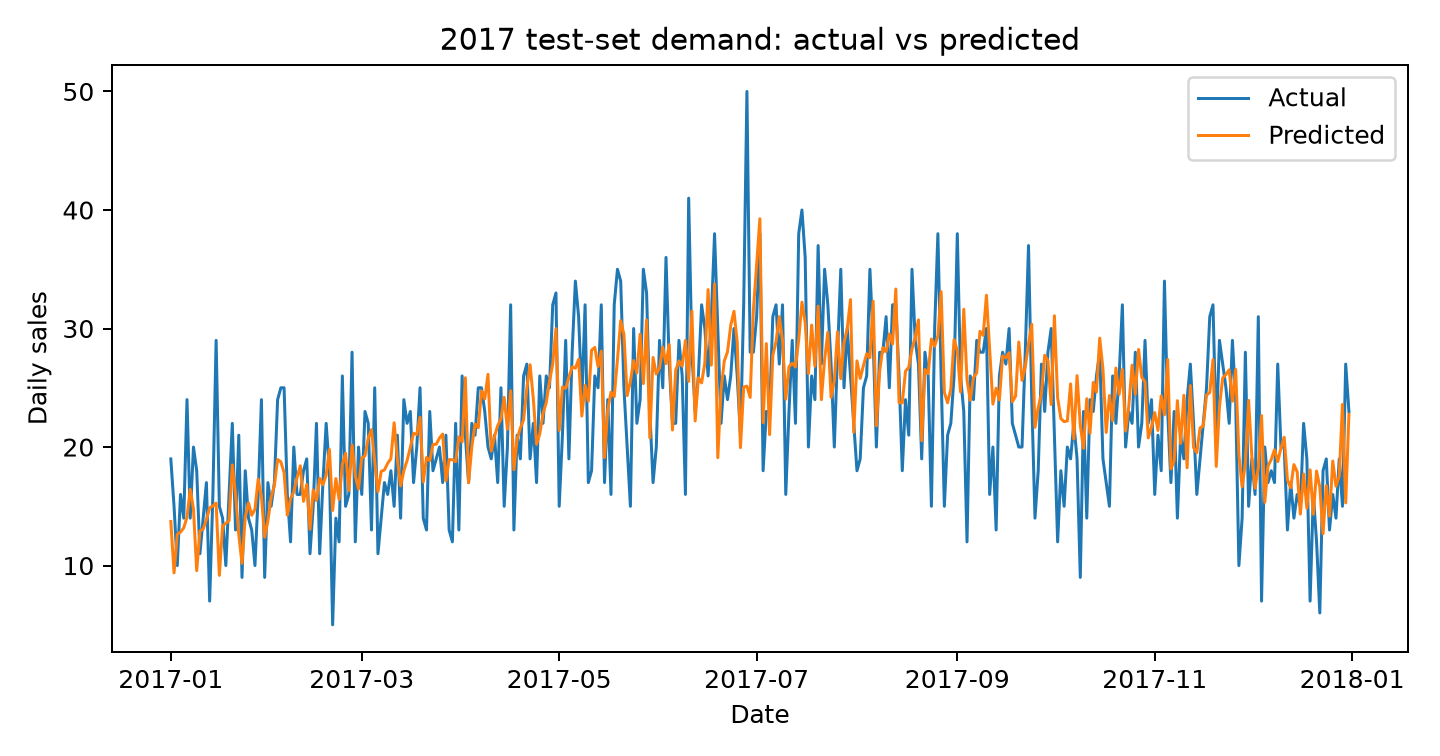
\includegraphics[width=0.82\textwidth]{../figures/fig8_actual_vs_predicted.png}
\caption{Actual versus predicted demand on the 2017 test set for the best main optimizer.}
\end{figure}

\section{Conclusion}
Polynomial regression can model useful nonlinear demand patterns when calendar and lag features are included. However, degree selection is critical: degree 2 generalized best in this experiment, while degrees 4 and 5 overfit strongly. L2 regularization improved generalization. For optimization, acceleration reduced training objective faster than plain Gradient Descent, proximal methods handled the non-smooth L1 objective, and adaptive stochastic methods provided an additional comparison relevant to machine learning practice.

\section*{Reproducibility}
Run \texttt{python src/main.py} from the project root. The implementation uses only NumPy, pandas, and matplotlib.

\section*{References}
Course task: \emph{Final Project - Optimization Methods for Polynomial Regression}. Lecture notes: \emph{Optimization for Data Science}, Christian Clason, University of Graz. Dataset: Kaggle Store Item Demand Forecasting Challenge.

\end{document}
